% ILS
% version 2022
%-------------------------------------------------------

\subsection{Introdución}
\label{06.01.introduccion}

Los sistemas de aproximación de aterrizaje son aquellos que proporcionan una guía al piloto de
una aeronave que desciente, para facilitarle la aproximación y aterrizaje a la pista del aeropuerto que
desea. Estos están normalizados según el tipo de pista, la OACI distingue entre:

\begin{itemize}
\item Pista de vuelo visual y
\item Pista de vuelo por instrumentos o Pista para aproximaciones de precisión
\end{itemize}

Se debe diferenciar entre aproximación y aterrizaje.

\begin{description}
\item [Aproximación:] consiste en una fase
de vuelo que comienza en el momento que se deja el vuelo de crucero para iniciar la maniobra de
acercamiento con descenso y finaliza en el momento en que se llega al punto de decisión, definido
como aquel en que se debe determinar si se aterriza o se frustra la maniobra, para elevarse de nuevo.

\item[Aterrizaje:]  es la operación que empieza en el punto de decisión, cuando ya se ha
  decidido tomar tierra y no se puede frustrar el aterrizaje, finalizando cuando la aeronave
  se ha posado en la pista, disminuyendo su velocidad hasta el punto de no poder abandonarla.
\end{description}

Una aproximación correcta conduce a un aterrizaje exitoso, por lo que son interdependientes uno
del otro.

La maniobra de aproximación suele dividirse en tres fases:

\begin{description}
\item [Aproximación inicial:] establece la transición entre vuelo de
  crucero y configuración de descenso. Se modifican los parámetros
  de velocidad y altura a la aproximación, los sistemas de navegación
  empleados son VOR, TACAN o ADF. Desde el control de tierra se puede
  ordenar modificar la trayectoria.
  
\item [Aproximación intermedia:] se
  siguen empleando los sistemas de navegación en el crucero, per la
  altitud, velocidad y distancia de separación con otras aeronaves
  cobran una relevancia especial. Esta fase termina en el punto en que
  se puede empezar a emplear el sistema de navegación de aproximación
  (PAR, ILS y MLS) con seguridad.
  
\item [Aproximación final:] en esta fase la
  aeronave ha interceptdo los haces del sistema de aproximación y
  está prácticamente alineada con la pista. La fase finaliza con el
  avión, ya posado en la pista, se encuentra con velocidad segura para
  abandonarla.
\end{description}

Para el caso del uso de instrumentos para la aproximación la OACI establece un procedimiento respectivo.


Los distintos sistemas disponibles para estas maniobras pueden ser clasificados según la forma de transmitir la información:

\begin{itemize}
\item Ayudas visuales
  \begin{itemize}
  \item Sistemas de Luces de Aproximación
  \item Sistema  Indicador de Pendiente de Aproximación Visual
  \item Indicador de Trayectoria de Aproximación de Precisión
  \end{itemize}
\item Ayudas radioeléctricas
\end{itemize}

\subsection{Requerimientos normativos}
\label{sec:06.requerimientos.normativos.aproximacion}


\begin{tcolorbox}[title={
Pista de vuelo visual.     
    OACI. Anexo 14. Edición 2018
  }
  ]
  {\footnotesize
    Pista destinada a las operaciones de aeronaves que utilicen procedimientos de aproximación visual
    o un procedimiento de aproximación por instrumentos a un punto más allá del cual pueda continuarse
    la aproximación en condiciones meteorológicas de vuelo visual.

\emph{Nota. Las condiciones meteorológicas de vuelo visual (VMC) se describen en el Capítulo 3 del Anexo 2 — Reglamento
del aire.
}
  }
  
\end{tcolorbox}


\begin{tcolorbox}[title= {Pista de vuelo por instrumentos o Pista para aproximaciones de precisión.
    OACI. Anexo 14. Edición 2018}]
  
  {\footnotesize

    Uno de los siguientes tipos de pista destinados a la operación de aeronaves que utilizan
    procedimientos de aproximación por instrumentos:
    
    \begin{enumerate}[a)]
    \item Pista para aproximaciones que no son de precisión. Pista de vuelo servida por ayudas visuales y ayudas no visuales
destinada a operaciones de aterrizaje después de una operación de aproximación por instrumentos de Tipo A y con
visibilidad no inferior a 1000 m.
\item Pista para aproximaciones de precisión de Categoría I. Pista de vuelo servida por ayudas visuales y ayudas no
visuales destinadas a operaciones de aterrizaje después de una operación de aproximación por instrumentos de Tipo B
con una altura de decisión (DH) no inferior a 60 m (200 ft) y con una visibilidad de no menos de 800 m o con un
alcance visual en la pista no inferior a 550 m.
\item Pista para aproximaciones de precisión de Categoría II. Pista de vuelo servida por ayudas visuales y ayudas no
visuales destinadas a operaciones de aterrizaje después de una operación de aproximación por instrumentos de Tipo B
con una altura de decisión (DH) inferior a 60 m (200 ft) pero no inferior a 30 m (100 ft) y con un alcance visual en la
pista no inferior a 300 m.
\item Pista para aproximaciones de precisión de Categoría III. Pista de vuelo servida por ayudas visuales y ayudas no
visuales destinada a operaciones de aterrizaje después de una operación de aproximación por instrumentos de Tipo B
hasta la superficie de la pista y a lo largo de la misma; y

\begin{enumerate}[A ]
\item Destinada a operaciones con una altura de decisión (DH) inferior a 30 m (100 ft), o sin altura de decisión y un
alcance visual en la pista no inferior a 175 m.
\item Destinada a operaciones con una altura de decisión (DH) inferior a 15 m (50 ft), o sin altura de decisión, y un
alcance visual en la pista inferior a 175 m pero no inferior a 50 m.
\item Destinada a operaciones sin altura de decisión (DH) y sin restricciones de alcance visual en la pista.
\end{enumerate}

\end{enumerate}

\emph{Nota 1. Las ayudas visuales no tienen necesariamente que acomodarse a la escala que caracterice las ayudas no visuales que se proporcionen. El criterio para la selección de las ayudas visuales se basa en las condiciones en que se trata de operar. \\
Nota 2. Consúltese el Anexo 6,  Operación de aeronaves, para los tipos de operaciones de aproximación por
instrumentos.
}

  }
\end{tcolorbox}


\begin{tcolorbox}[title={Procedimiento de aproximación por instrumentos (IAP). OACI Anexo 6. Edición 2018}]
  {\footnotesize

    Serie de maniobras predeterminadas realizadas por referencia a los instrumentos de a bordo, con protección específica contra los obstáculos desde el punto de referencia de aproximación inicial, o, cuando sea el caso, desde el inicio de una ruta definida de llegada hasta un punto a partir del cual sea posible hacer el aterrizaje; y, luego, si no se realiza éste, hasta una posición en la cual se apliquen los criterios de circuito de espera o de margen de franqueamiento de obstáculos en ruta. Los procedimientos de aproximación por instrumentos se clasifican como sigue:
    
    \begin{description}
    \item [Procedimiento de aproximación que no es de precisión, \ac{NPA}]. Procedimiento de aproximación por instrumentos diseñado para operaciones de aproximación por instrumentos 2D de Tipo A.

\emph{Nota. Los procedimientos de aproximación que no son de precisión pueden ejecutarse aplicando la técnica de
Aproximación Final en Descenso Continuo, \ac{CDFA}. Las \ac{CDFA} con guía \ac{VNAV} de asesoramiento, calculada por el equipo de
a bordo se consideran operaciones de aproximación por instrumentos 3D. Las \ac{CDFA} con cálculo manual de la velocidad
vertical de descenso requerida se consideran operaciones de aproximación por instrumentos 2D. En los PANS-OPS
(Doc 8168), Volumen I, Parte II, Sección 5, se proporciona más información sobre las CDFA.
}

\item [Procedimiento de aproximación con guía vertical (APV)]. Procedimiento de aproximación por instrumentos, con
navegación basada en la performance (PBN), diseñado para operaciones de aproximación por instrumentos 3D de
Tipo A.

\item[ Procedimiento de aproximación de precisión (PA)]. Procedimiento de aproximación por instrumentos, basado en sistemas
de navegación (ILS, MLS, GLS, y SBAS CAT I), diseñado para operaciones de aproximación por instrumentos 3D de
Tipo A o B.

\emph{Nota. Véase la Sección II, Capítulo 2, 2.2.8.3, en relación con los tipos de operación de aproximación por instrumentos.}

\end{description}
  }
\end{tcolorbox}

\begin{tcolorbox}
  {\footnotesize

    \begin{description}
      
\item[2.2.8.3] Las operaciones de aproximación por instrumentos se clasificarán basándose en los mínimos de utilización más
bajos por debajo de los cuales la operación de aproximación deberá continuarse únicamente con la referencia visual requerida,
de la manera siguiente:

\begin{enumerate}[a)]
\item \textbf{Tipo A:} una altura mínima de descenso o altura de decisión igual o superior a 75 m (250 ft); y
\item \textbf{Tipo B:} una altura de decisión inferior a 75 m (250 ft). Las operaciones de aproximación por instrumentos de Tipo B están categorizadas de la siguiente manera:
  \begin{enumerate}[1)]
  \item  \textbf{Categoría I (CAT I):} una altura de decisión no inferior a
    60 m (200 ft) y con visibilidad no inferior a 800 m o alcance
    visual en la pista no inferior a 550 m; 
  \item \textbf{Categoría II (CAT II):}
    una altura de decisión inferior a 60 m (200 ft), pero no inferior
    a 30 m (100 ft) y alcance visual en la pista no inferior a 300 m;
    
  \item \textbf{Categoría IIIA (CAT IIIA):} una altura de decisión inferior a 30
    m (100 ft) o sin limitación de altura de decisión y alcance visual
    en la pista no inferior a 175 m; 
  \item \textbf{Categoría IIIB (CAT IIIB):} una
    altura de decisión inferior a 15 m (50 ft) o sin limitación de
    altura de decisión y alcance visual en la pista inferior a 175 m
    pero no inferior a 50 m; y 
  \item \textbf{Categoría IIIC (CAT IIIC):} sin
    altura de decisión ni limitaciones de alcance visual en la pista.
\end{enumerate}

\end{enumerate}

\emph{Nota 1. Cuando los valores de la altura de decisión (DH) y del alcance visual en la pista (RVR) corresponden a
categorías de operación diferentes, la operación de aproximación por instrumentos ha de efectuarse de acuerdo con los
requisitos de la categoría más exigente (p. ej., una operación con una DH correspondiente a la CAT IIIA, pero con un RVR de
la CAT IIIB, se consideraría operación de la CAT IIIB, o una operación con una DH correspondiente a la CAT II, pero con un
RVR de la CAT I, se consideraría operación de la CAT II).\\
Nota 2. La referencia visual requerida significa aquella sección de las ayudas visuales o del área de aproximación que
debería haber estado a la vista durante tiempo suficiente para que el piloto pudiera hacer una evaluación de la posición y de la rapidez del cambio de posición de la aeronave, en relación con la trayectoria de vuelo deseada. En el caso de una operación de aproximación en circuito, la referencia visual requerida es el entorno de la pista.
}

\end{description}
}
\end{tcolorbox}



\begin{figure}[!htb]
  \centering
  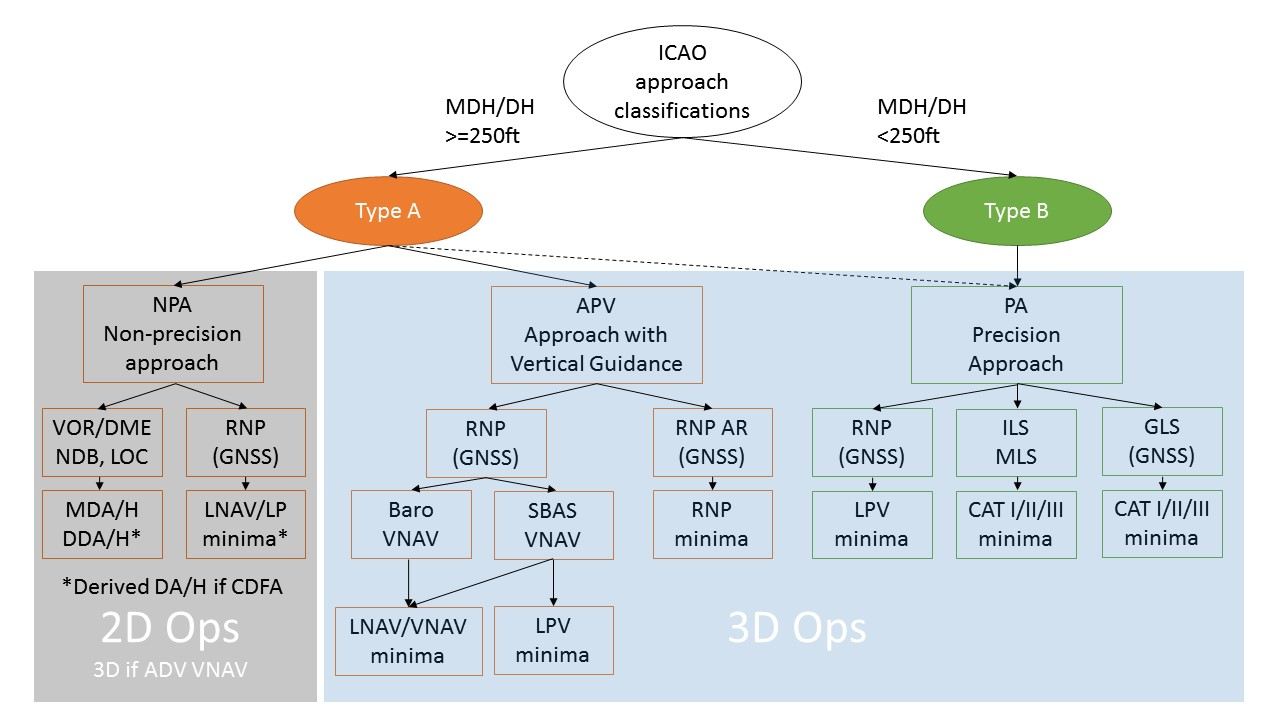
\includegraphics[width=0.9\textwidth]{06.radionavegacion/Imagenes/OACI-Doc8168-tiposInstrumentosAproximacion.jpg} 
  \caption{Tipos de instrumentos para aproximación según OACI \protect\cite{NuevasAproximaciones}}
  \label{fig:06.tipos.instrumentos.aproximacion}
\end{figure}


\begin{table}[!htb]
  \centering
  \caption[06.OACI.requisitos.]{OACI Requisitos de performance en apoyo de las operaciones de aproximación por instrumentos}
  \label{tab:06.OACI.requisitos}

  \begin{tabular}{lm{0.3\linewidth}m{0.2\linewidth}} \hline 
    \multicolumn{2}{c}{Performance de sistemas en el Anexo 10}
    & {Método del Anexo 6 - Categoría de operación de aproximación}
    \\ \hline 
    Aproximación que no es de precisión (NPA)
    &
    &2D-Tipo A$^1$
    \\ \hline
    Aproximación con guía vertical (APV)
    &
    &3D-Tipo A$^2$
    \\ \hline
    Aproximación de precisión (PA)
    & Categoría I, DH igual o superior a 75 m (250 ft)
    &3D-Tipo A$^3$ \\ \cline{2-3}
    & Categoría I, DH igual o superior a 60 m (200
      ft) e inferior a 75 m (250 ft)
    & 3D-Tipo B - CAT I $^3$ \\ \cline{2-3}
    & Categoría II
    & 3D-Tipo B - CAT II \\ \cline{2-3}
    & Categoría II
    & 3D-Tipo B - CAT II \\  \hline
    \multicolumn{3}{l}{\footnotesize
    \parbox{\linewidth}{
        $^1$ Sin  guía vertical barométrica \\
    $^2$ Con guía vertical barométrica o SBAS \\
    $^3$ Con guía vertical ILS, MLS, GBAS o SBAS.
    }	
    } \\
  \end{tabular}
\end{table}

\href{https://skybrary.aero/sites/default/files/bookshelf/2991.pdf}{OACI Doc 9613
  Performance-Based Navigation Manual}


\subsection{Ayudas visuales}
\label{sec:06.02.ayudasvisuales}


Las ayudas visuales utilizan la energía electromagnética como portadora de información y permiten
realizar con mayor eficacia el contacto visual con la pista de aterrizaje y con la trayectoria
correcta de la senda de descenso.

Son dispositivos luminosos cromáticos que emplean el contraste para
transmitir la información al piloto.

Como es lógico, estas ayudas son indispensables en aterrizajes
nocturnos o diurnos de baja visibilidad.

En cuanto a las características que las ayudas visuales  presentan son  descritas
por lo que se denomina las ``\emph{5C}'': 

\begin{description}
  
\item [Configuración] se refiere a la forma de emplazamiento de las
unidades que componen cualquier sistema de ayuda visual iluminada, especificando distancias
entre ellas, distancias respecto al umbral de pista (sector desde donde se inicia el área destinada a
las operaciones aéreas), etc.

\item[Color] los colores según norma utilizados para diferenciar las señales de las ayudas visuales iluminadas.

\item[Cobertura] se refiere a los sectores en los que son visibles las ayudas visuales iluminadas y a la reducción del
  deslumbramiento.
  
\item[Candelas] unidad de intensidad lumínica, las recomendaciones que la OACI emite son
curvas de isocandelas las cuales deben cumplirse y que varía de acuerdo a la posición y función
de las ayudas visuales iluminadas (diagramas publicados en el Anexo 14).

Se sabe que la agudeza visual y la sensibilidad frente al deslumbramiento varían según las
personas, la edad de ellas y el grado de fatiga.  Un elemento importante para el deslumbramiento
es la transmitibilidad atmosférica, que varía cuando es de día, atardecer, noche o cuando
existe niebla.

Para otorgar un buen servicio, dentro las operaciones aéreas, a los pilotos evitando los
problemas de deslumbramiento, los reguladores de corriente constante poseen un rango de
variación de intensidad lumínica (variación de brillo) que depende de las características de las
ayudas visuales.

Por lo general las luces de alta y media intensidad posee de 3 a 5 niveles de intensidad, en cambio
las luces de baja intensidad solo posee un solo nivel de intensidad.

\item[Continuidad] las ayudas visuales más críticas deben tener un alto grado de continuidad en la
emisión de sus señales, por lo que se tienen dos circuitos eléctricos en las luces de borde de pista
y luces de aproximación, en caso de falla de uno de ellos el otro se mantiene operable y aun son
visibles las señales luminosas.

\end{description}




\subsubsection{Sistemas de Luces de Aproximación}
\label{sec:06.02.01.ALS}

El Sistema de Luces de Aproximación (ALS,  Approach Light Systems) se utiliza en aeródromos
con alta frecuencia de uso. Se ubican en las cercanias de la cabecera de la pista como parte a las
ayudas electrónicas de navegación para la parte final de aproximaciones precisas y no precisas de un
vuelo IFR, y también como una guía visual en vuelos VFR nocturnos.
En la Figura \ref{fig:06.ALS.aeropuerto} puede observarse el ALS de la aproximación a la pista 27
del aeropuerto Liverpool - John Lennon.

El ALS suministra al piloto con entradas visuales respecto a la alineación de la aeronave, el
balance, el horizonte, el ancho y la posición con respecto a la cabecera de la pista. Desde que los
sistemas de iluminación aeroportuarios relevaron a las necesariamente rápidas acciones mentales
sobre la información visual que encabezaban las decisiones, un sistema visual es ideal para una guía
durante los últimos segundos críticos del movimiento descendente sobre el patrón de planeo.

El sistema de luces de aproximación se creó en base al ángulo del patrón de planeo, el rango visual,
el ángulo de visibilidad cortada en la cabina y de las velocidades de aterrizaje. Esto es esencial para
que los pilotos estén propensos a utilizar e identificar ALS y de interpretar el sistema sin confusión.
El sistema comienza en el umbral de cabecera de pista y se extiende hacia el frente de la misma por,
aproximadamente, 900 m (3000 pies). En caso de que esta longitud no pueda ser utilizada, se emplea
la mayor posible. Una columna de luces estroboscópicas de alta intensidad luminosa, alimentadas
mediante una descarga de condensador e igulamente espaciadas, se coloca alineada con el eje de la
pista y al ser accionadas producen un efecto de flash que indica a los pilotos la ubicación del centro
de la pista en condiciones de baja visibilidad.

En los Estados Unidos de América los ALS poseen una Fila de Decisión (Decision Bar), ubicada
a 1000 pies (300 m) de la cabecera de pista, la cual sirve como un horizonte visible para facilitar
la transición de IFR a VFR. También se la ubica de forma que coincida con la Altura de Decisión
(Decision Altitude).

\begin{tcolorbox}[title={Requerimientos OACI. Anexo 14. Volumen I. Edición 2018.
    }]
{\footnotesize
  \begin{description}
  \item [5.3.4.1]  Aplicación
    \begin{enumerate}[A ]
    \item {\bf Pista de vuelo visual}
      
      Recomendación. Cuando sea materialmente posible, debería instalarse un sistema sencillo de iluminación de aproximación tal como el que se especifica en 5.3.4.2 a 5.3.4.9, para servir a una pista de vuelo visual cuando el número de clave sea 3 ó 4 y destinada a ser utilizada de noche, salvo cuando la pista se utilice solamente en condiciones de buena visibilidad y se proporcione guía suficiente por medio de otras ayudas visuales.
      
{\it Nota. También puede instalarse un sistema sencillo de iluminación de aproximación para proporcionar guía visual
  durante el día.}

\item {\bf  Pista para aproximaciones que no son de precisión}
  
Cuando sea materialmente posible, se instalará un sistema sencillo de iluminación de aproximación, tal como el que se
especifica en 5.3.4.2 a 5.3.4.9, para servir a una pista para aproximaciones que no son de precisión, salvo cuando la pista se
utilice solamente en condiciones de buena visibilidad y se proporcione guía suficiente por medio de otras ayudas visuales.

\emph{Nota. Es conveniente que se considere la posibilidad de instalar un sistema de iluminación de aproximación de
precisión, de Categoría I, o la adición de un indicador que lleve a la pista.}

\item \textbf{ Pista para aproximaciones de precisión de Categoría I}
  
Cuando sea materialmente posible, en una pista para aproximaciones de precisión de Categoría I se instalará un sistema de
iluminación de aproximación de precisión de Categoría I, tal como el que se especifica en 5.3.4.10 a 5.3.4.21.

\item \textbf{ Pista para aproximaciones de precisión de Categorías II y III}
  
En una pista para aproximaciones de precisión de Categorías II y III, se instalará un sistema de iluminación de
aproximación de precisión de las Categorías II o III, tal como se especifica en 5.3.4.22 a 5.3.4.39.


\end{enumerate}
\end{description}
}
\end{tcolorbox}




Diversas configuraciones de ALS son reconocidas por la OACI, sin embargo, configuraciones no
normalizadas se encuentran instaladas en diversos aeropuertos. Los ALS son sistemas de luces de alta
intensidad y varios se complementan con otros ubicados sobre la senda de aproximación, tal como el
Runway End Identifier Lights (REIL), Touchdown Zone Lights (TDZL), and High Intensity Runway
Lights (HIRL). Entre las configuraciones más usuales se tienen:

{\footnotesize
\begin{description}
\item[MALSR:] Medium-intensity Approach
Lighting System with Runway Alignment
Indicator Lights

\item[MALSF:] Medium-intensity Approach
Lighting System with Sequenced Flashing
lights

\item[SALS:] Simple Approach Lighting System

\item[SSALS:] Simplified Short Approach Lighting System

\item[SSALR:] Simplified Short Approach Light-
ing System with Runway Alignment Indicator Lights

\item[ODALS:] Omnidirectional Approach Lighting System
  
\item[ALSF-1:] Approach Lighting System with
  Sequenced Flashing Lights configuration 1
  
\item[ALSF-2:] Approach Lighting System with
  Sequenced Flashing Lights configuration 2
  
\item[CALVERT I/ICAO-1 HIALS:] ICAO-compliant configuration 1 High Intensity
  Approach Lighting System
  
\item[CALVERT II/ICAO-2 HIALS:] ICAO-compliant configuration 2 High Intensity
  Approach Lighting System
  
\item[LDIN:] Lead-in lighting
  
\item[REIL:] Runway End Identification Lights

\item[RAIL:] Runway Alignment Indicator Lights

\end{description}
}

En las configuraciones que poseen luces secuenciadas (sequenced flashing lights), estas son de tipo
estroboscópicas y se ubican de frente a la cabecera de pista, sobre el eje de la misma. Estas luces
se encienden en secuencia, comenzando con la luz más distante de la cabecera y terminando en la
Fila de Decisión (Decision Bar). Esto se justifica para no distraer al piloto durante la fase crítica de cambiar de IFR a VFR. El sistema de luces secuenciadas es comunmente conocido como ``\emph{el conejo}'' (the rabbit) o ``\emph{correr al conejo}'' (the running rabbit).

\begin{figure}[!htb]
  \centering
  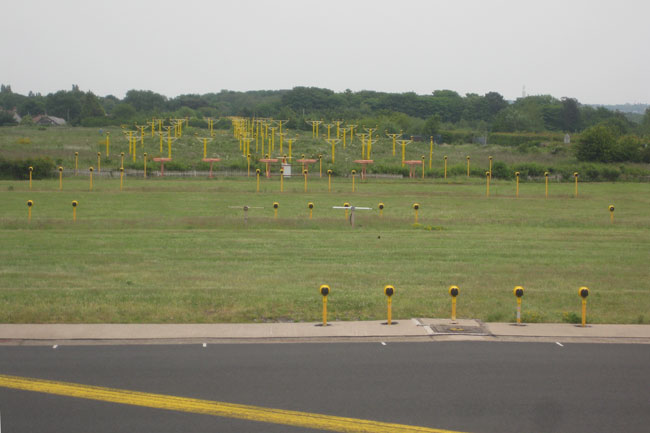
\includegraphics[width=0.9\textwidth]{06.radionavegacion/Imagenes/06.ALS/ALS-01.jpg} 
  \caption{ALS \protect\cite{ALSfoto}}
  \label{fig:06.ALS.aeropuerto}
\end{figure}



\subsubsection{Sistema  Indicador de Pendiente de Aproximación Visual }
\label{sec:06.02.02.VASIS}


\begin{tcolorbox}[title=Requerimientos OACI. Anexo 14. Volumen I. Edición 2018.
  5.3.5 Sistemas visuales indicadores de pendiente de aproximación]

  {\footnotesize

    \begin{description}
    \item [5.3.5.1] Se instalará un sistema visual indicador de pendiente de aproximación para facilitar la aproximación a una pista, que cuente o no con otras ayudas para la aproximación, visuales o no visuales, cuando exista una o más de las condiciones
siguientes:
\begin{enumerate}[a)]
\item La pista sea utilizada por turborreactores u otros aviones
  con exigencias semejantes en cuanto a guía para la aproximación; 
\item el piloto de cualquier tipo de avión pueda tener dificultades para
  evaluar la aproximación por una de las razones siguientes:

  \begin{enumerate}[1)]
  \item orientación visual insuficiente, por ejemplo, en una
    aproximación de día sobre agua o terreno desprovisto de puntos de
    referencia visuales o durante la noche, por falta de luces no
    aeronáuticas en el área de aproximación; o 
  \item información visual
    equívoca, debida por ejemplo, a la configuración del terreno
    adyacente o a la pendiente de la pista;
\end{enumerate}
\item la presencia de objetos en el área de aproximación pueda constituir un peligro grave si un avión desciende por debajo de la trayectoria normal de aproximación, especialmente si no se cuenta con una ayuda no visual u otras ayudas visuales que adviertan la existencia de tales objetos;
\item las características físicas del terreno en cada extremo de la pista constituyan un peligro grave en el caso en que un avión efectúe un aterrizaje demasiado corto o demasiado largo; y
\item las condiciones del terreno o las condiciones meteorológicas predominantes sean tales que el avión pueda estar sujeto a turbulencia anormal durante la aproximación.
\end{enumerate}
\item[5.3.5.2] Los sistemas visuales indicadores de pendiente de aproximación normalizados consistirán en lo siguiente:
  \begin{enumerate}[a)]
  \item  T-VASIS y AT-VASIS que se ajusten a las especificaciones
    contenidas en 5.3.5.7 a 5.3.5.23 inclusive; 
  \item PAPI y APAPI que se
    ajusten a las especificaciones contenidas en 5.3.5.24 a 5.3.5.41
    inclusive; según se indica en la Figura xxx.
  \end{enumerate}
  
\item [5.3.5.3] Se instalarán PAPI, T-VASIS o AT-VASIS si el número de clave es 3 ó 4 o cuando existe una o más de las condiciones especificadas en 5.3.5.1.
    \end{description}
}


\end{tcolorbox}


El Sistema Indicador de Pendiente de Aproximación Visual ( VASIS, Visual
Approach Slope Indicator System) es un sistema de luces al costado de la pista que provee información
de guía visual para el aterrizaje durante la aproximación a una pista. Estas luces pueden ser avistadas
desde una distancia de hasta 5 nm ($\approx  9$ km) durante el día y desde hasta 20 nm ($\approx  37$ km) o más
de noche.

Este sistema posee diversas variantes:

\begin{description}

\item[VASIS Estándar:] consiste en varios conjuntos de 2, 4, 6, 12 o 16 luces dispuestas en filas y
denominadas near, middle y far. La mayoría de las instalaciones VASIS consisten en conjuntos
de 2 filas, near y far, y poseen conjuntos de 2, 4 o 12 luces. Otros VASIS tienen 3 filas, near,
middle y far, lo que permite al piloto con diferentes pendientes de aproximación. Esta última
instalación puede tener de 6 a 16 luces. Las instalaciones VASIS de 2, 4 o 6 luces se ubican a un
lado de la pista, usualmente la izquierda desde el punto de vista del piloto. Las instalaciones
de 12 a 16 luces se colocan en cantidades iguales a ambos lados de la pista.

Las instalaciones VASIS de 2 filas proveen una única pendiente de aproximación, usualmente,
a 3º.

Las instalaciones de 3 filas proveen dos pendientes de aproximación. La pendiente
inferior es indicada por la fila near y middle, usualmente, a 3 grados; la pendiente superior
es guiada por las filas middle y far, y es, aproximadamente, 1/4º mayor. Esta última
pendiente se utiliza en aviones con cabina alta. La pendiente normal del dispositivo es de tres
grados, en algunos lugares se indican pendientes de 4,5º para evitar obstaculos en la
aproximación. El uso de pendientes superiores a 3,5º puede causar un incremento en la
longitud de pista requerida.

Cada conjunto de luces está diseñado de tal manera que las luces se ven o blancas o rojas, de-
pendiendo del ángulo al cual las luces son vistas. Cuando el piloto está aterrizando en el ángulo
de aproximación apropiado, lo que significa que se encuentra en la trayectoria de aproximación
correcta, el primer conjunto de luces se ven blancas y el segundo conjunto, rojas. Cuando am-
bos conjuntos se ven blancos, esto significa que está volando demasiado alto; y demasiado bajo
cuando ambos se ven rojos.

Este es el tipo más común de sistema de indicación de pendiente
de aproximación visual.

\item[PVASIS:] ( Pulsating Visual Approach Slope Indicator System) es una
luz única al costado de la pista de aterrizaje. Se ve blanco fijo cuando se está en la correcta
trayectoria de aproximación, parpadeante blanco por encima y rojo fijo cuando se encuentra
por debajo de la trayectoria de aproximación. Esta última empieza a parpadear cada vez más
rápido cuanto más se aleja la aeronave de la trayectoria de aproximación ideal.

Este tipo de
Indicador de Pendiente de Aproximación Visual es raramente utilizado en parte porque son
facilmente confundidos con otras luces de la pista.

\item[VASIS Tricolor:] Consiste en una luz única que se ve de color ámbar por sobre la trayectoria
de aproximación ideal, blanca en la trayectoria correcta y roja debajo de él. También es muy
poco utilizada, en cierta medida debido a que se sabe que los pilotos que no están familiarizados
con él han malinterpretado las luces, provocando una ``\emph{corrección}'' en la dirección equivocada.

\item[T-VASIS:] (T Visual Approach Slope Indicator System) 
  Consiste en una barra perpendicular al eje de la pista
con 4 luces y una barra paralela al eje de la pista con 6 luces, y que intersecta a la anterior en
el punto medio. Éste esquema se repite en ambos lados de la pista en el T-VASIS,
ver Figura \ref{fig:06.sistemas.indicadores.pendiente.aproximacion}.

La instalación completa de T-VASIS ocupa un espacio considerable según la Figura \ref{fig:T-VasisAeropuerto} 
de la pista 32 del aeropuerto de Brisbane en agosto de 2007.
Las instalaciones de T-VASIS se han resaltado a ambos lados de la pista, se encuentran dentro de la franja de la pista.
Se puede distinguir cada caja de luz individual dentro del sistema
en la Figura \ref{fig:T-VasisCajaLuz} 
se observa un primer plano de una caja de luz del sistema. En la Figura \ref{fig:T-VasisLayout}
se observa el layout según OACI.

Cuando la aeronave va con la inclinación correcta solamente se
verá la barra transversal y su color será blanco, si va por encima de la senda de planeo correcta
verá la barra transversal y también algunas de las luces centrales que están por encima de la
barra transversal, todas ellas de color blanco. Mientras se vuele más por arriba, más luces
centrales se verán.
Si la aeronave va por debajo de la senda, se verá la barra transversal y algunas de las luces
centrales que están por debajo de la barra, todas ellas de color blanco. Si está MUY por debajo,
verá estas mismas luces pero de color rojo. En la Figura 
puede verse lo anteriormente explicado.

\item[AT-VASIS:] Abbreviated T Visual Approach Slope Indicator System, similar al anterior 
consistiendo en 10 elementos luminosos dispuestos a un lado de la pista en forma de una sola barra
de ala de cuatro luces cortada en su punto medio por una fila longitudinal de seis luces,
ver Figura \ref{fig:06.sistemas.indicadores.pendiente.aproximacion}.

\end{description}

\begin{figure}[!htb]
  \centering
  \includegraphics[width=0.7\textwidth]{06.radionavegacion/Imagenes/06.VASIS/06-TVasis+AT-Vasis+Papi+Apapi.pdf}
  \caption{ Sistemas visuales indicadores de pendientes de aproximación \protect\cite{Anexo14Vol1}}
  \label{fig:06.sistemas.indicadores.pendiente.aproximacion}
\end{figure}

\begin{figure}[!htb]
  \centering
  \subfigure[T-Vasis en aeropuerto \protect\cite{T-VasisAeropuerto}]{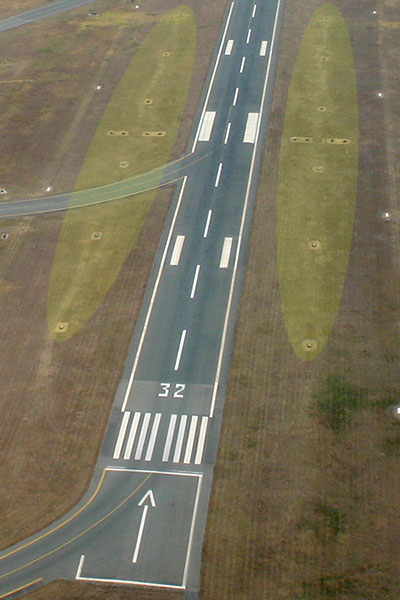
\includegraphics[width=0.4\textwidth]{06.radionavegacion/Imagenes/06.VASIS/BN-32-14-showing-T-VASIS-1-8-07.jpg} \label{fig:T-VasisAeropuerto} }
\qquad
\subfigure[T-Vasis caja de luz \protect\cite{T-VasisCajaLuz}]{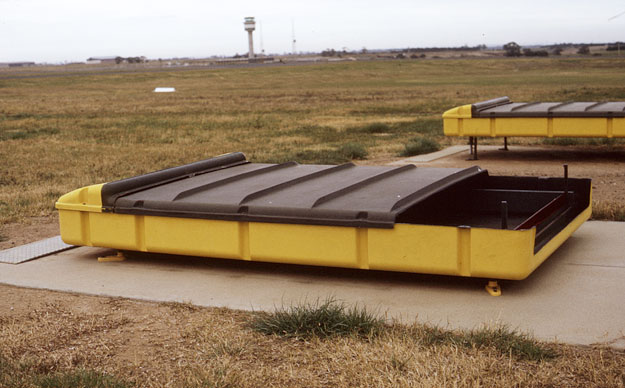
\includegraphics[width=0.4\textwidth]{06.radionavegacion/Imagenes/06.VASIS/Melbourne-T-VASIS-Type-B-bar-box-8-72-CAHS-Byron-Sullivan.jpg} \label{fig:T-VasisCajaLuz} }

\subfigure[T-Vasis Layout \protect\cite{Anexo14Vol1}]{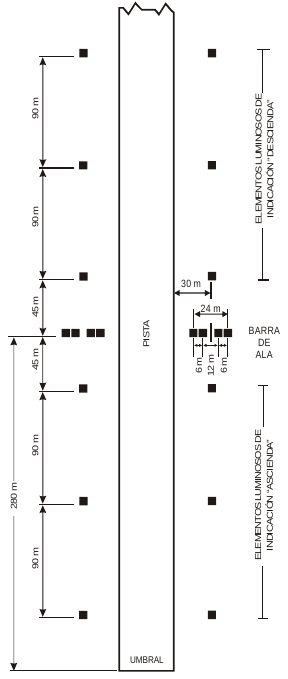
\includegraphics[angle=-90, width=0.9\textwidth]{06.radionavegacion/Imagenes/06.VASIS/06-T-Vasis-emplazamientoOACI.png} \label{fig:T-VasisLayout} }

  \caption{T-Vasis}
  \label{fig:t-vasis}
\end{figure}



\begin{tcolorbox}[title={OACI, Anexo 14. Volumen I. Edición 2018.} ]

  \begin{description}
  \item[5.3.5.2] Los sistemas visuales indicadores de pendiente de aproximación normalizados consistirán en lo siguiente:
    \begin{enumerate}[a)]
    \item  T-VASIS y AT-VASIS que se ajusten a las especificaciones
      contenidas en 5.3.5.7 a 5.3.5.23 inclusive; 
    \item  PAPI y APAPI que  se ajusten a las especificaciones contenidas en 5.3.5.24 a
      5.3.5.41 inclusive; según se indica en la Figura xxxx.
\end{enumerate}
\item[5.3.5.3] Se instalarán PAPI, T-VASIS o AT-VASIS si el número de clave es 3 ó 4 o cuando existe una o más de las
condiciones especificadas en 5.3.5.1. 
  \end{description}

\end{tcolorbox}  

\begin{tcolorbox}[colback=red!5!white, colframe=red!75!black,fonttitle=\bfseries,
  title={OACI, Anexo 14. Volumen I. Edición 2018.}]
  \begin{description}
  \item [5.3.5.4 Recomendación.] A partir del 1 de enero de 2020,
    debería discontinuarse el uso de T-VASIS y AT-VASIS como sistemas
    indicadores de pendiente en aproximación visual.
\end{description}

\end{tcolorbox}


\subsubsection{Indicador de Trayectoria de Aproximación de Precisión}
\label{sec:06.02.03.PAPI}

También conocido como PAPI (Precision Approach Path Indicator), es un sistema más moderno de indicación
de pendiente de aproximación.

Fué desarrollado en 1974 por Tony Smith y David Johnson de la Royal Aircraft Establishment en Bedford, Inglaterra,
siendo necesarios más de dos años para su completa operatividad, que se remonta a mediados del año 1977
cuando se puso a prueba en el aeropuerto de Gatwick en Londres el prototipo de un sistema visual de aproximación
que proporcionaba datos de la senda de planeo (el primer PAPI).

%Fabricado por ADB, se observó que sus señales eran más precisas que las del sistema VASIS existente hasta el momento, que era operativo hasta unos 200 pies frente a los  50 pies del PAPI.

Consiste en cuatro conjuntos de luces alineados en forma perpendicular a la pista de aterrizaje.
Funciona básicamente del mismo modo en que lo hace el VASIS estándar, pero las luces adicionales
indican al piloto que tan alejado de la trayectoria de aproximación ideal se encuentra la aeronave.
En la Figura \ref{fig:PAPI.layout} se observa el layout según OACI.

Cuando los dos conjuntos de luces más alejados se ven rojos y los más cercanos blancos,
la aeronave está exactamente en la trayectoria de aproximación.
Cuando los tres conjuntos de luces más
alejados se ven rojos, se encuentra apenas por debajo, mientras que si los tres conjuntos de luces
más próximos se ven blancos, la aeronave está apenas por encima de la trayectoria de aproximación.
Cuatro conjuntos de luces rojas indican que está muy por debajo de la trayectoria de aproximación,
y cuatro conjuntos de luces blancas indican que está muy por encima. La mayoría de los aeropuertos
importantes utilizan este sistema.

El PAPI es colocado generalmente del lado izquierdo de la pista de aterrizaje/despegue y puede
ser visto desde una distancia máxima de 5 nm durante el día y a una distancia máxima de
20 nm de noche. Tiene dos o cuatro cajas de luces colocadas en una única fila, lo que lo
diferencia del VASIS que tiene dos filas: una más próxima y otra más alejada.

Cada caja de luces está equipada con un mecanismo óptico que divide la luz emitida en dos
segmentos, rojo y blanco. Dependiendo del ángulo de aproximación, las luces se verán o rojas o
blancas desde la posición del piloto. Lo ideal sería que las luces visibles se muevan entre el rango de
todas blancas y de la mitad rojas, cambiando a rojo sucesivamente de derecha a izquierda. El piloto
alcanza la normal trayectoria de aproximación (generalmente de 3º) cuando la mitad de las
luces sean rojas y la otra mitad blancas. Si está por debajo de la trayectoria de aproximación, las
luces rojas sobrepasarán en cantidad a las blancas, si está por encima, observará más luces blancas.

El PAPI se basa en el principio de la Lente de Fresnel.

El estándar para el PAPI de la FAA es el mismo que corresponde al VASIS OACI.

\href{https://adbsafegate.com/documents/2116/en/manual-voltage-powered-papi}{Manual ADB Safegate de PAPI}


\begin{figure}[!htb]
  \centering
  \subfigure[Papi layout \protect\cite{Anexo14Vol1}]{
    \includegraphics[width=0.9\textwidth]{06.radionavegacion/Imagenes/06.PAPI/PapiLayoutOACI.pdf}
    \label{fig:PAPI.layout}
    }
  \caption{PAPI}
  \label{fig:06.papi}
\end{figure}



\subsection{Ayudas radioeléctricas}
\label{sec:06.03.ayudas.radioelectricas}

Entre las ayudas radioeléctricas, la que se ha utilizado por los últimos sesenta años y se encuentra
normalizada por la OACI, es el ILS. En algunos aeropuertos, sobre todo militares, es complementado
con un sistema radárico denominado PAR.
%El ILS esta siendo sustituido por el MLS que proporciona prestaciones superiores.

